\section{Envelope}
\subsection{Walls} % Andrew
\paragraph{Wall Construction Type}
First, we selected the general types of wall construction methods to be represented in ComStock. We chose the four general wall types commonly used in commercial building energy codes because they cover the most common wall construction types and can be linked to nominal thermal characteristics. The definitions of these types from \cite{ashrae_901_2010} are as follows, with the corresponding ComStock enumerations shown in parentheses:

\begin{itemize}
\item \textbf{Mass wall} (Mass): A wall with a heat capacity exceeding (1) 7 Btu/ft\textsuperscript{2}·F or (2) 5 Btu/ft\textsuperscript{2}·F, provided that the wall has a material unit weight not greater than 120 lb/ft\textsuperscript{3}.
\item \textbf{Metal building wall} (Metal Building): A wall whose structure consists of metal spanning members supported by steel structural members (i.e., does not include spandrel glass or metal panels in curtain wall systems).
\item \textbf{Steel-framed wall} (SteelFramed): A wall with a cavity (insulated or otherwise) whose exterior surfaces are separated by steel  framing members (i.e., typical steel stud walls and curtain wall systems).
\item \textbf{Wood-framed and other walls} (WoodFramed): All other wall types, including wood stud walls.
\end{itemize}

To determine the prevalence of each wall construction type, we queried a database, \cite{lightbox_smartparcels_2021}, containing  building type, number of stories, location, and wall construction. The database did not use the same wall construction types selected for ComStock, so we created a mapping between the database entries and the wall construction types listed above, as shown in Table~\ref{tab:wall_construction_mapping}. Some construction types in the database were excluded from the mapping, either because the meaning was ambiguous or because they represented an insignificant fraction of the entries in the database. The excluded constructions represent only 5\% of the total samples, with 4.5\% labeled “OTHER” (which there was no clear way to map).

Upon reviewing the data, we identified two instances that were likely misclassifications. The first was buildings higher than five stories with the wall construction type``WoodFramed''. Historically, it was not possible to use WoodFramed construction for buildings over five stories, and even today, this practice is uncommon. Buildings with this combination were reassigned to ``Mass'' walls, based on the assumption that people were observing large wood internal structural members in old buildings and classifying them as WoodFramed. The second was buildings higher than two stories with ``MetalBuilding'' walls. Based on experience, this construction technique is commonly reserved for 1--2 story buildings only. Buildings with this combination were reassigned to ``SteelFramed,'' based on the assumption that this would be the most likely alternative classification if a person observed steel structural elements.

After mapping each entry in the database to one of the ComStock construction types, we analyzed the data to determine other building characteristics in the database were correlated with construction type. Older buildings were slightly more likely to use mass constructions, but the change over time was minor. Construction type varied significantly as a function of the number of stories. Shorter buildings were much more likely to be wood-framed, whereas taller buildings were more likely to be mass, and very tall buildings were likely to be steel-framed (steel studs or curtain wall). Based on a spot-checking of the database, we found the building type classification to be less reliable than other building characteristics. Although there was some correlation between building type and wall construction, there was also a correlation between building type and number of stories. Because of the joint correlation, we selected number of stories instead of building type. There was a clear correlation between climate zone and construction type---most notably, there was a much lower incidence of mass walls in cold climate zones. There was some correlation between construction type and building floor area. However, there was also a correlation between the number of stories and the building area. Because the construction type is physically limited by a building's height, it was more logical to use the number of stories as a driving characteristic for construction type. Following this analysis, we concluded that the number of stories and climate zone should be used as drivers of wall construction type. The probabilities for each combination of number of stories and climate zone were calculated  and then used as the input distribution for wall construction type in ComStock. This distribution is summarized in Table~\ref{tab:wall_constuction_types}.

\paragraph{Wall System Turnover Rate}
As described in Section~\ref{sec:system_turnover_and_eul}, we assume that some building systems, including exterior walls, are replaced over the lifespan of the building. Typically, for exterior walls, the structural elements of the wall are maintained, while the cladding, insulation, sheathing, etc. are be replaced. As noted in Section~\ref{sec:system_turnover_and_eul}, the EUL for exterior walls is assumed to be 200 years, which means that most buildings are modeled with the walls they were built with. Once the wall construction type probabilities and distributions of building types, sizes, and vintages are carried through the sampling process and simulations are created, the distribution of construction types and energy code levels can be reviewed. As shown in Figure~\ref{fig:weighted_floor_area_by_energy_code_and_wall_type}, because the majority of the building stock is older, and wall systems are replaced at a low rate, most of the building floor area is assumed to have walls that follow the oldest energy codes.

\begin{figure}[ht!] \centering
    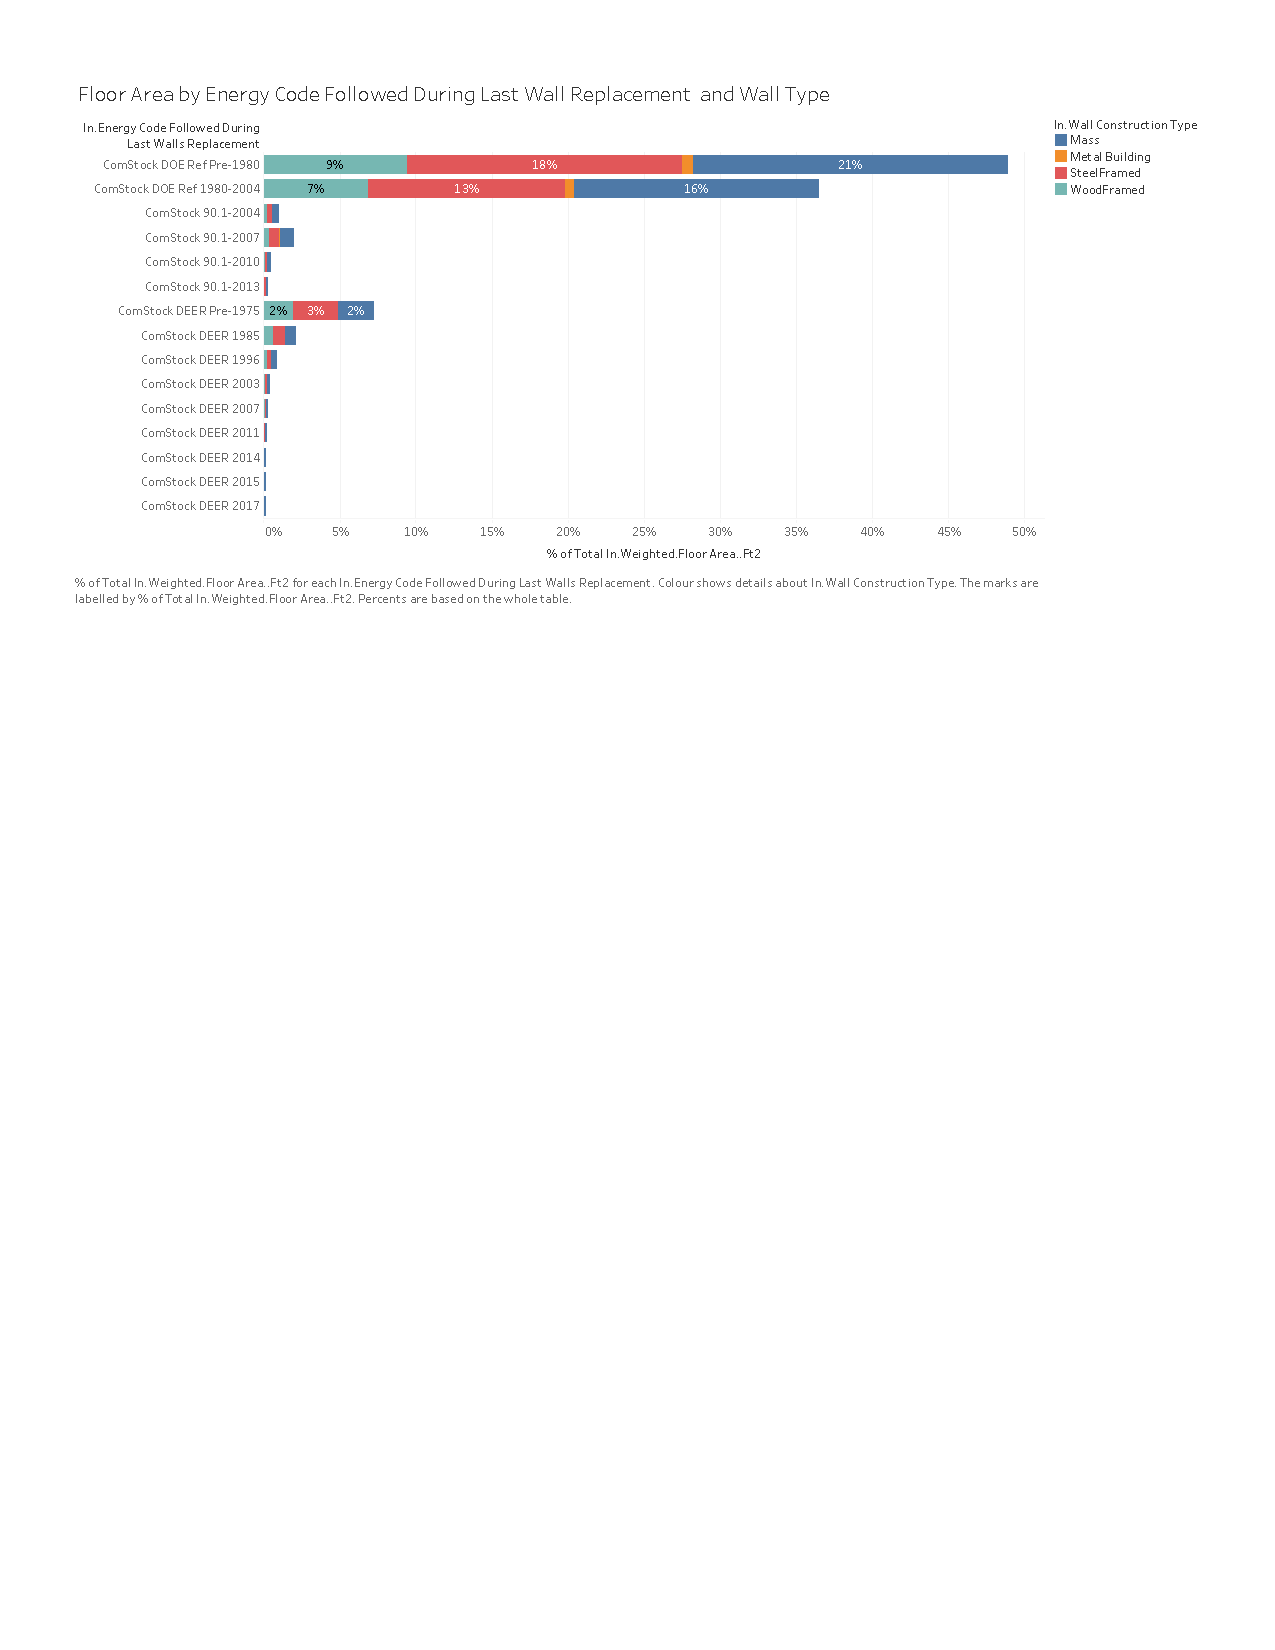
\includegraphics[
        page={1},
        trim={1cm 18.3cm 1cm 1cm}, clip, % L B R T
        width=\textwidth]{figures/docs_envelope.pdf}
    \caption[Weighted floor area by energy code followed during last wall replacement and wall type]{Weighted floor area by energy code followed during last wall replacement and wall type.}
    \label{fig:weighted_floor_area_by_energy_code_and_wall_type}
\end{figure}
\vspace{2mm}
\paragraph{Wall Thermal Performance}
We did not find any data sources that contained the thermal performance (U-Value/R-Value) of walls in the commercial building stock. This is likely because surveys would need to either find building plans, which can be difficult or impossible for older buildings, or disassemble part of the structure to look inside the walls, which building owners are unlikely to allow. To account for the lack of data, we estimated wall thermal performance based on an estimate of the energy code followed when the wall was last replaced. Section~\ref{sec:energy_code} describes how the energy code was determined. The thermal performance of walls for each energy code varies based on climate zone and construction type, as shown in Table~\ref{tab:wall_r_values} and Table~\ref{tab:wall_r_values_deer}. Note that although these thermal performance values do include the thermal bridging inherent in the clear field wall, they do not include thermal bridging at intermediate floors, parapets, and glazing transitions. These additional thermal bridges are expected to lower the overall thermal performance of the wall assembly.

As previously described, most of the building stock's walls are assumed to be older. Therefore, the thermal performance assumptions for older vintages have a much higher impact on the overall heating and cooling demand than those for newer vintages. The ComStock DOE Ref Pre-1980 assumptions, taken from \cite{doe_reference_buildings}, are originally from a study of only offices \citep{old_vintage_office_study}. Unfortunately, this study no longer appears to be available. Following the methodology in \cite{doe_reference_buildings}, these values are used for all wall construction types and all building types. Figure~\ref{fig:weighted_floor_area_by_building_type_and_wall_type} shows the final prevalence of each wall construction type by building type. Most notable is the low prevalence of metal building walls across the stock, even in warehouses. This might be surprising, but it is supported by the available data. Table \ref{tab:wall_r_value_averages} shows the average wall thermal performance by ASHRAE Standard 169--2006 climate zone.

\begin{figure}[ht!] \centering
    \includegraphics[
        page={2},
        trim={1cm 20.7cm 1cm 1cm}, clip, % L B R T
        width=\textwidth]{figures/docs_envelope.pdf}
    \caption[Weighted floor area by wall type and building type]{Weighted floor area by wall type and building type.}
    \label{fig:weighted_floor_area_by_building_type_and_wall_type}
\end{figure}

\vspace{2mm}

\subsection{Windows} % Andrew
\paragraph{Window Construction Type}
Data from the NFRC Commercial Fenestration Market Study was used to develop the modeling approach for windows in ComStock. This study, conducted by Guidehouse in collaboration with NFRC, characterized the national commercial window stock through data collection and analysis. Six primary data sources representing all regions of the United States were used in the study---a 2020 Guidehouse survey, NEEA CBSA, DOE Code Study, CAEUS, CBECS, and RECS. A variety of window properties were collected, including the window-to-wall ratio, number of panes, frame material, glazing type, low-E coating, gas fill, solar heat gain coefficient (SHGC), U-factor, and many others. In total, the database contained approximately 16,000 samples, each with an appropriate weighting factor based on the coverage, completeness, and fidelity of each data source. The WWR data was already incorporated into the ComStock baseline during the EULP project. Some of the other key window properties such as thermal performance were then used to create the new baseline window constructions and distributions discussed later in this section. A summary of the data sources and their associated information is shown in Table ~\ref{tab:window_data_sources}.

Four window properties---number of panes, glazing type, frame material, and low-E coating---were used to create the baseline window configurations. These four parameters were selected based on which characteristics have the most impact on window performance, which have the most data available from the various data sources, and which inputs we trust from the average building owner or survey recipient. The options for each property are shown in Figure \ref{fig:window_configurations}.

\begin{figure}[ht!] \centering
    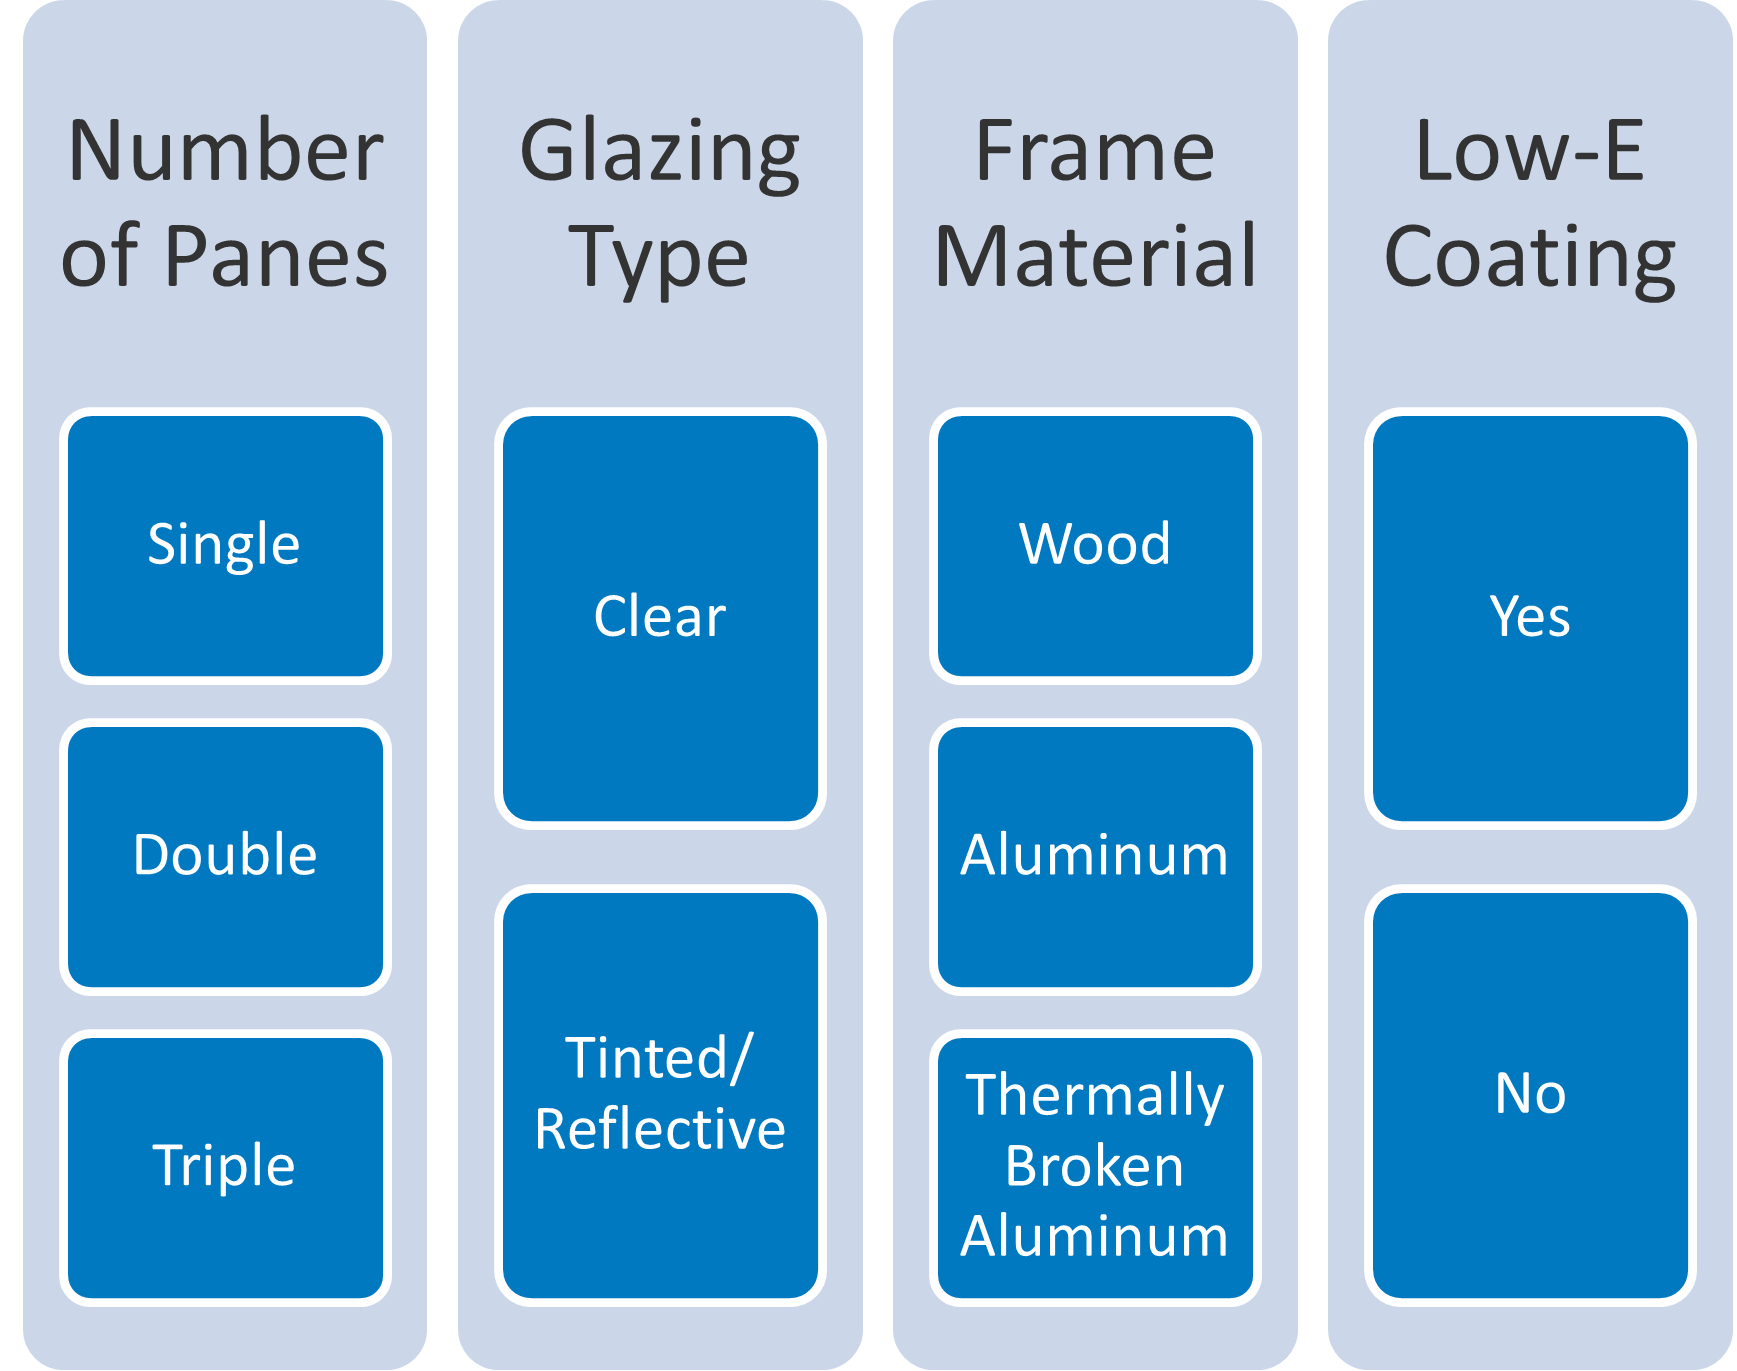
\includegraphics[
        trim={0cm 0cm 0cm 0cm}, clip, % L B R T
        width=0.5\textwidth]{figures/window_configurations.png}
    \caption{Window characteristics for number of panes, glazing type, frame material, and low-E coating.}
    \label{fig:window_configurations}
\end{figure}
\vspace{5mm}

Modeling every combination of these four properties would result in 36 different window configurations, which would add significant complexity to the sampling process. Instead, we selected 12 combinations to be modeled, based on which combinations are most common and most realistic. There are four single-pane, six double-pane, and two triple-pane configurations. The unrealistic/uncommon combinations that were eliminated include:
\begin{itemize}
\item Single pane with thermally broken aluminum frame
\item Single pane with low-E coating
\item Double pane with wood frame
\item Triple pane with no low-E coating
\item Triple pane without thermally broken aluminum frame
\item Thermally broken double or triple pane without low-E coating.
\end{itemize}
The 12 remaining window configurations are shown in Table \ref{tab:window_configurations}.

\begin{table}
\centering
\caption[Window Configurations]{Window Configurations}
\label{tab:window_configurations}
\begin{tabular}{|l|l|l|l|}
\hline
\textbf{Number of Panes} & \textbf{Glazing Type} & \textbf{Frame Material} & \textbf{Low-E Coating} \\ \hline
Single          & Clear             & Aluminum                    & No            \\ \hline
Single          & Tinted/Reflective & Aluminum                    & No            \\ \hline
Single          & Clear             & Wood                        & No            \\ \hline
Single          & Tinted/Reflective & Wood                        & No            \\ \hline
Double          & Clear             & Aluminum                    & No            \\ \hline
Double          & Tinted/Reflective & Aluminum                    & No            \\ \hline
Double          & Clear             & Aluminum                    & Yes           \\ \hline
Double          & Clear             & Aluminum With Thermal Break & Yes           \\ \hline
Double          & Tinted/Reflective & Aluminum                    & Yes           \\ \hline
Double          & Tinted/Reflective & Aluminum With Thermal Break & Yes           \\ \hline
Triple          & Clear             & Aluminum With Thermal Break & Yes           \\ \hline
Triple          & Tinted/Reflective & Aluminum With Thermal Break & Yes           \\ \hline
\end{tabular}
\end{table}

We created a sampling distribution for the new window constructions for the entire country using the initial data set. Overall, single-pane windows make up approximately 54\% of the stock, double-pane windows make up 46\%, and triple-pane windows make up <1\%. Initially, we created distributions based on census division to incorporate geographic location into the sampling. Upon further analysis, we found that it was also necessary to incorporate the energy codes into distributions to prevent scenarios where a single-pane window was sampled for a certain location, but, according to the energy code for that location, a double-pane window was required. For this reason, we modified the sampling distribution to include two dependencies---climate\_zone and  energy\_code\_followed\_during\_last\_window\_replacement.

To generate these sampling distributions, we used the maximum U-values specified for each climate zone in each version of ASHRAE 90.1, using climate zones defined by ASHRAE 169--2006. For each combination of climate zone and energy code, the 12 window configurations were evaluated to determine which were both realistic and met code (i.e., had a U-value lower than the code maximum U-value). For the older energy codes, we made several assumptions about technology adoption to determine which window configurations were realistic:
\begin{itemize}
    \item Low-E coating---not adopted until DOE Ref 1980--2004
    \item Thermally broken aluminum frame---not adopted until 90.1-2004
    \item Triple pane---not adopted until 90.1-2004.
\end{itemize}

Each combination of climate zone and energy code included 2--12 window configurations that met the criteria. After limiting the distributions to these configurations, we renormalized the percentages from the national distribution to 100\%. This kept the percentages from the national distribution while also incorporating intelligent assumptions based on climate zone and energy code. Table ~\ref{tab:window_distribution_4A} provides an example of the window configurations that were sampled for each code year in climate zone 4A.

\begin{table}
\scriptsize
\centering
\caption[Window Distribution Assumptions Example]{Window Distribution Assumptions Example from Climate Zone 4A}
\label{tab:window_distribution_4A}
\begin{tabular}{p{2.5in}|rrrrrr}
\textbf{Energy Code Followed During Last Windows Replacement}                      & \textbf{Pre-1980} & \textbf{1980-2004} & \textbf{90.1-2004} & \textbf{90.1-2007} & \textbf{90.1-2010} & \textbf{90.1-2013} \\
\textbf{Allowable Assembly Maximum U-Value}                                        & 1.22              & 0.59               & 0.57               & 0.55               & 0.55               & 0.42  \\
\textbf{Allowable Assembly Maximum SHGC}                                           & 0.54              & 0.36               & 0.39               & 0.4                & 0.4                & 0.4   \\ \hline
Single - No LowE - Clear - Aluminum \- U-1.178 SHGC-0.744                            & X                 &                    &                    &                    &                    &       \\ \hline
Single - No LowE - Tinted/Reflective - Aluminum \- U-1.178 SHGC-0.579                 & X                 &                    &                    &                    &                    &       \\ \hline
Single - No LowE - Clear - Wood \- U-0.91 SHGC-0.683                                  & X                 & X                  &                    &                    &                    &       \\ \hline
Single - No LowE - Tinted/Reflective - Wood \- U-0.91 SHGC-0.525                      & X                 & X                  &                    &                    &                    &       \\ \hline
Double - No LowE - Tinted/Reflective - Aluminum \- U-0.749 SHGC-0.484                 & X                 & X                  &                    &                    &                    &       \\ \hline
Double - No LowE - Clear - Aluminum \- U-0.746 SHGC-0.646                             & X                 & X                  &                    &                    &                    &       \\ \hline
Double - LowE - Clear - Aluminum \- U-0.559 SHGC-0.386                                &                   & X                  & X                  & X                  & X                  &       \\ \hline
Double - LowE - Tinted/Reflective - Aluminum \- U-0.557 SHGC-0.274                    &                   & X                  & X                  & X                  & X                  &       \\ \hline
Double - LowE - Clear - Thermally Broken Aluminum \- U-0.499 SHGC-0.378               &                   &                    & X                  & X                  & X                  & X     \\ \hline
Double - LowE - Tinted/Reflective - Thermally Broken Aluminum \- U-0.496 SHGC-0.266   &                   &                    & X                  & X                  & X                  & X     \\ \hline
Triple - LowE - Clear - Thermally Broken Aluminum \- U-0.3 SHGC-0.328                 &                   &                    & X                  & X                  & X                  & X     \\ \hline
Triple - LowE - Tinted/Reflective - Thermally Broken Aluminum \- U-0.299 SHGC-0.224   &                   &                    & X                  & X                  & X                  & X \\ \hline
& \multicolumn{6}{l}{X = This window type meets code minimums} \\
\end{tabular}
\end{table}

As can be seen in Table \ref{tab:window_distribution_4A}, for DOE Ref Pre-1980, the only windows that met code and are realistic are single-pane or double-pane windows with no low-E coating. For DOE Ref 1980--2004, the maximum U-value dropped significantly, such that single-pane aluminum windows no longer met code. However, double-pane low-E windows became available on the market at that time. For 90.1-2004 through 90.1-2010, code required a U-value equivalent to double-pane low-E or better, and in 90.1-2013, the code improved again, meaning that double-pane low-E with a thermal break or better was required. This type of logic was applied to all combinations of climate zone and energy code. Then, we converted the data into the distributions used in sampling.

A small adjustment was made to the final distributions because some states and localities do not follow or enforce energy codes strictly. Following the code exactly would likely overestimate window performance. Therefore, in scenarios where single-pane windows were technically below code, we assumed that 5\% of all windows in the stock would still have the worst-performing single-pane windows installed. The distributions were adjusted accordingly by subtracting 5\% total from the double-pane configurations and adding to the single-pane aluminum configurations. After making this manual adjustment, the new distributions had the same overall breakdown as the national distribution generated from the Guidehouse data---54\% single-pane and 46\% double-pane .

\paragraph{Window Thermal Performance}
Once the 12 new window constructions were determined, a team from Lawrence Berkeley National Laboratory's (LBNL’s) Windows and Daylighting Group used the WINDOW program to assign thermal performance properties to each construction. SimpleGlazing objects in EnergyPlus were chosen to represent windows to reduce complexity. This choice also simplifies the process of applying upgrades, because all fenestration objects in the baseline models use the same object type. The inputs for the SimpleGlazing object are U-factor, solar heat gain coefficient (SHGC), and visible light transmittance (VLT). For each window configuration, LBNL assigned a frame ID and window ID from the WINDOW database. They also filled in the respective U-factors, SHGCs, and VLTs, which are shown in Table \ref{tab:window_thermal_performance}.

The U-factors originally ranged from U-1.18 Btu/h·ft\textsuperscript{2}·F for the worst-performing single-pane window to U-0.30 Btu/h·ft\textsuperscript{2}·F for the best-performing triple-pane window. As mentioned earlier in this section, the maximum U-Factor that EnergyPlus can model with a simple glazing object is U-1.02 Btu/h·ft\textsuperscript{2}·F, which is governed by the limitations of a 2D heat transfer model when interior and exterior air films are included. Therefore, we adjusted the U-factor for the first two single-pane windows to be U-1.02 Btu/h·ft\textsuperscript{2}·F rather than U-1.18 Btu/h·ft\textsuperscript{2}·F. This allowed these windows to be modeled in ComStock. This results in a slight overestimate of the thermal performance of single-pane windows.


\subsection{Roof} % Andrew
\paragraph{Roof Construction Type}
First, we reviewed the general types of roof construction methods that could be represented. The three general roof types commonly used in commercial building energy codes were chosen because they cover the most common roof construction types and can be linked to nominal thermal characteristics. The definitions of these types from \cite{ashrae_901_2010} are as follows:

\begin{itemize}
\item \textbf{Roof with insulation entirely above deck (IEAD)}: A roof that has all insulation installed above (outside of) the roof structure and that is continuous (i.e., uninterrupted by framing members).
\item \textbf{Metal building roof}: A roof that is constructed with a metal, structural weathering surface; has no ventilated cavity; and has the insulation entirely below deck (i.e., does not include composite concrete and metal deck construction or a roof framing system that is separated from the superstructure by a wood substrate). In addition, the roof structure consists of one or
more of the following configurations: (a) metal roofing in direct contact with the steel framing members, (b) metal roofing separated from the steel framing members by insulation, or (c) insulated metal roofing panels installed as described in a or b.
\item \textbf{Attic and other roof}: All other roofs, including roofs with insulation entirely below (inside of) the roof structure (e.g., attics, cathedral ceilings, and single-rafter ceilings); roofs with insulation both above and below the roof structure; and roofs without insulation (excluding metal building roofs).
\end{itemize}

The analysis of roof properties in \cite{eia2012cbecs}, shown in Figure~\ref{fig:cbecs_floor_area_by_roof_tilt_and_attic_presence}, indicates that about 90\% of the commercial floor space covered by ComStock has flat or shallow pitch roofs, and that the large majority of the buildings with flat or shallow pitch roofs do not have attic space. Given these factors and the complexity associated with modeling the geometry of pitched roofs, we decided to model the entire stock as having flat roofs.

\begin{figure}[h] \centering
    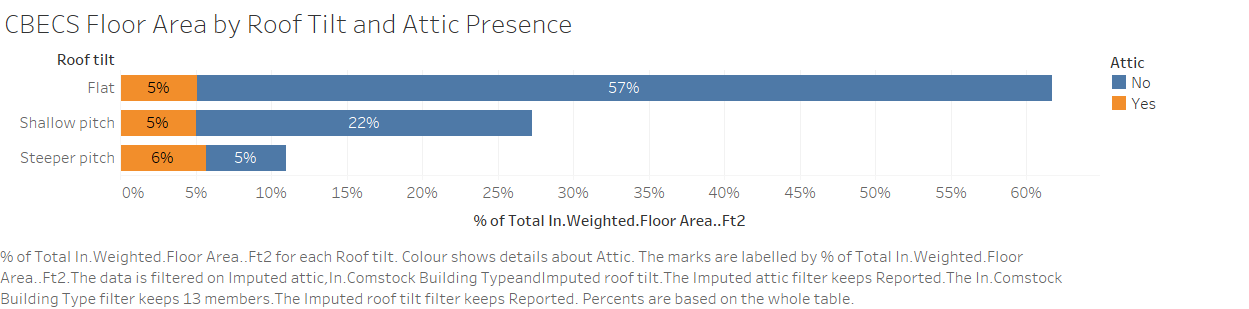
\includegraphics[
        trim={0cm 1.5cm 0cm 0cm}, clip, % L B R T
        width=\textwidth]{figures/cbecs_floor_area_by_roof_tilt_and_attic_presence.png}
    \caption{Weighted floor area by roof tilt and attic presence.}
    \label{fig:cbecs_floor_area_by_roof_tilt_and_attic_presence}
\end{figure}

\vspace{5mm}
No data sources for roof construction type were found. For buildings outside of California, a single roof construction type was chosen for each building type. As shown in Table~\ref{tab:roof_construction_types}, most buildings are assumed to use IEAD roofs, which is consistent with the assumption of flat roofs. For buildings in California, the construction types from the DEER prototype buildings were used \citep{cpuc_deer}.

\paragraph{Roof System Turnover Rate}
As described in Section \ref{sec:system_turnover_and_eul}, some building systems, including roofs, are assumed to be replaced over the lifespan of the building. Typically, for roofs, the structural elements are maintained, while the roof membrane and insulation are replaced. As noted in Section \ref{sec:system_turnover_and_eul}, the EUL for roofs was assumed to be 200 years, which means that most buildings are modeled with the roof insulation they were built with. Once the roof type probabilities and distribution of building types, sizes, and vintages are carried through the sampling process and simulations are created, the distribution of energy code levels can be reviewed. As shown in Figure~\ref{fig:weighted_floor_area_by_energy_code_roofs}, because the majority of the building stock is older, and roof systems are replaced at a low rate, most of the building floor area is assumed to have roofs that follow the oldest energy codes.

\begin{figure}[h] \centering
    \includegraphics[
        page={3},
        trim={1cm 20.5cm 1cm 1cm}, clip, % L B R T
        width=\textwidth]{figures/docs_envelope.pdf}
    \caption{Weighted floor area by energy code followed during last roof replacement.}
    \label{fig:weighted_floor_area_by_energy_code_roofs}
\end{figure}
\vspace{5mm}
\paragraph{Roof Thermal Performance}
We did not find any data sources that contained the thermal performance (U-Value/R-Value) of roofs in the commercial building stock. This is likely because surveys would need to either find building plans, which can be difficult or impossible for older buildings, or disassemble part of the structure to look inside the roofs, which building owners are unlikely to allow. To account for the lack of data, we estimated roof thermal performance based on an estimate of the energy code followed when the roof was last replaced. Section~\ref{sec:energy_code} describes how the energy code was determined. The thermal performance of roofs for each energy code varies based on climate zone and construction type, as shown in Tables~\ref{tab:roof_r_values} and \ref{tab:roof_r_values_deer}. While these thermal performance values do include the thermal bridging inherent in the clear field roof, they do not include thermal bridging at parapets, skylight curbs, or roof penetrations for HVAC systems. These additional thermal bridges are expected to lower the overall thermal performance of the roof assembly.

As previously described, most of the building stock's roofs are assumed to be older. Therefore, the thermal performance assumptions for older vintages have a much higher impact on the overall heating and cooling demand than the assumptions for newer vintages. The ComStock DOE Ref Pre-1980 assumptions, taken from \cite{doe_reference_buildings}, are originally from a study of only offices \citep{old_vintage_office_study}. Unfortunately, this study no longer appears to be available. Following the methodology in \cite{doe_reference_buildings}, these values are used for all roof construction types and all building types.


\subsection{Floor}
In ComStock, all buildings are assumed to be built using slab-on-grade construction and to have no cantilevered thermal zones. Thus, the only heat transfer into the building through floors is assumed to happen through the floor in contact with the ground. All floors between stories are internal surfaces, and any heat transfer through these surfaces occurs between zones within the building, not between the building and the outside environment.

\paragraph{Floor Thermal Performance}
We did not find any data sources that contained the thermal performance of floors in the commercial building stock. This is likely because surveys would need to either find building plans, which can be difficult or impossible for older buildings, or excavate under a slab edge, which is impractical. To account for the lack of data, we estimated floor thermal performance based on an estimate of the energy code followed when building was first constructed. Section~\ref{sec:energy_code} describes how the energy code was determined. The thermal performance of floors for each energy code varies based on climate zone, as shown in Table~\ref{tab:floor_f_factors}. It is notable that only buildings built to the newest energy codes in the coldest climates assume any sort of slab insulation.

\subsection{Thermal Bridging} % Matthew Dahlhausen
Thermal bridging includes the impact of uninsulated structural elements that undermine the overall thermal resistance of an opaque assembly. These include linear thermal bridges, such as along corners, roof parapets, and fenestration, and point thermal bridges, such as protruding steel beams. These are formalized by psi factors multiplied by the length of a thermal bridge, and chi factors multiplied by the number of a thermal bridge. ASHRAE publishes psi and chi factors for common major thermal bridges, and thermal bridging requirements were recently added to the envelope section of ASHRAE 90.1-2022 \citep{ashrae_901_2022}. See Appendix section A10.2 of ASHRAE 90.1-2022 for details on calculating thermal bridges.

Thermal bridging in ComStock is implemented with the Thermal Bridging and Derating (TBD) ruby gem \citep{tbd_gem}. The gem detects the presence of common major thermal bridges in the model (corners, parapets, etc.), and derates the adjacent opaque surface construction (walls and roofs) to account for the thermal bridging. TBD gem version 3.4.1 includes default ASHRAE 90.1-2022 psi and chi factors for different kinds of thermal bridges. These vary by wall construction type (steel frame, mass, wood) and whether thermal bridges are considered mitigated or unmitigated. By default, ComStock assumed the unmitigated 90.1-2022 psi and chi factors by wall construction type. Specific values are listed in the TBD gem \citep{tbd_gem}.

\subsection{Infiltration and Natural Ventilation} % Matthew Dahlhausen

\subsubsection{Infiltration}
Infiltration in ComStock uses the same model as EnergyPlus \citep{energy_plus}, detailed in equation \ref{energyplus_infiltration_eqn}.

\begin{align}
\label{energyplus_infiltration_eqn}
Infiltration = I_{design} * F_{schedule} * [A + B * |(T_{zone} - T_{odb})| + C * WindSpeed + D * WindSpeed^2]
\end{align}

where:\\
\begin{itemize}
\item \textbf{I\textsubscript{design}} is the design infiltration flow rate, in m\textsuperscript{3} per s per m\textsuperscript{2} exterior surface area\\
\item \textbf{F\textsubscript{schedule}} is a fractional schedule, usually tied to HVAC system operation\\
\item \textbf{A} is the coefficient for constant infiltration\\
\item \textbf{B} is the coefficient for temperature difference driven infiltration\\
\item \textbf{T\textsubscript{zone}} is the zone air temperature, in degrees Celsius\\
\item \textbf{T\textsubscript{odb}}  is the outdoor dry bulb temperature, in degrees Celsius\\
\item \textbf{C} and \textbf{D} are linear and quadratic coefficients for wind driven infiltration\\
\item \textbf{WindSpeed} is the local windspeed, in m per s.\\
\end{itemize}

The selection of the design infiltration rate is somewhat arbitrary, as it depends on the assumed natural pressure at typical conditions. The coefficients need to be paired with an assumed natural pressure.

\subsubsection{Infiltration Rates}
Infiltration rates are calculated from measured airtightness data from \citep{nist_infiltration_data}. There are significant differences in building airtightness due to differences in wall construction, shown in Figure 6 of the NIST reference. Airtightness does not vary significantly by building type or vintage. Airtightness does depend on size, but this is inherently captured by larger buildings having smaller surface area to volume ratios. Air barriers greatly reduce leakiness, but they are rare in existing buildings, and only recently have been required in some jurisdictions. Airtightness of buildings in ComStock follow lognormal distributions with airtightness means by wall construction type matched to those in \citep{nist_infiltration_data}, shown in Figure \ref{fig:airtightness_by_wall_construction_type}.
Airtightness values are measured at 75 Pa and are 6-sided, meaning the infiltration is normalized by total building exterior surface area including wall, roof, and ground surfaces.

The design infiltration rate is calculated from the airtightness value assuming a 4 Pa design pressure, shown in \ref{airtightness_to_design_infiltration}
\begin{align}
\label{airtightness_to_design_infiltration}
I_{\text{design}} = \text{airtightness} \cdot \left(\frac{1\ \text{hr}}{3600\ \text{s}}\right) \cdot \left(\frac{5\ \text{sided area}}{6\ \text{sided area}}\right) \cdot \left(\frac{4.0\ \text{Pa}}{75.0\ \text{Pa}}\right)^{0.65}
\end{align}
where:\\
\begin{itemize}
\item \textbf{airtightness} is the measured airtightness at 75 Pa in m\textsuperscript{3} per hr per m\textsuperscript{2} 6-sided exterior surface area\\
\item \textbf{I\textsubscript{design}} is the design infiltration rate at 4 Pa in m\textsuperscript{3} per s per m\textsuperscript{2} 5-sided exterior surface area\\
\end{itemize}

\begin{figure}
    \centering 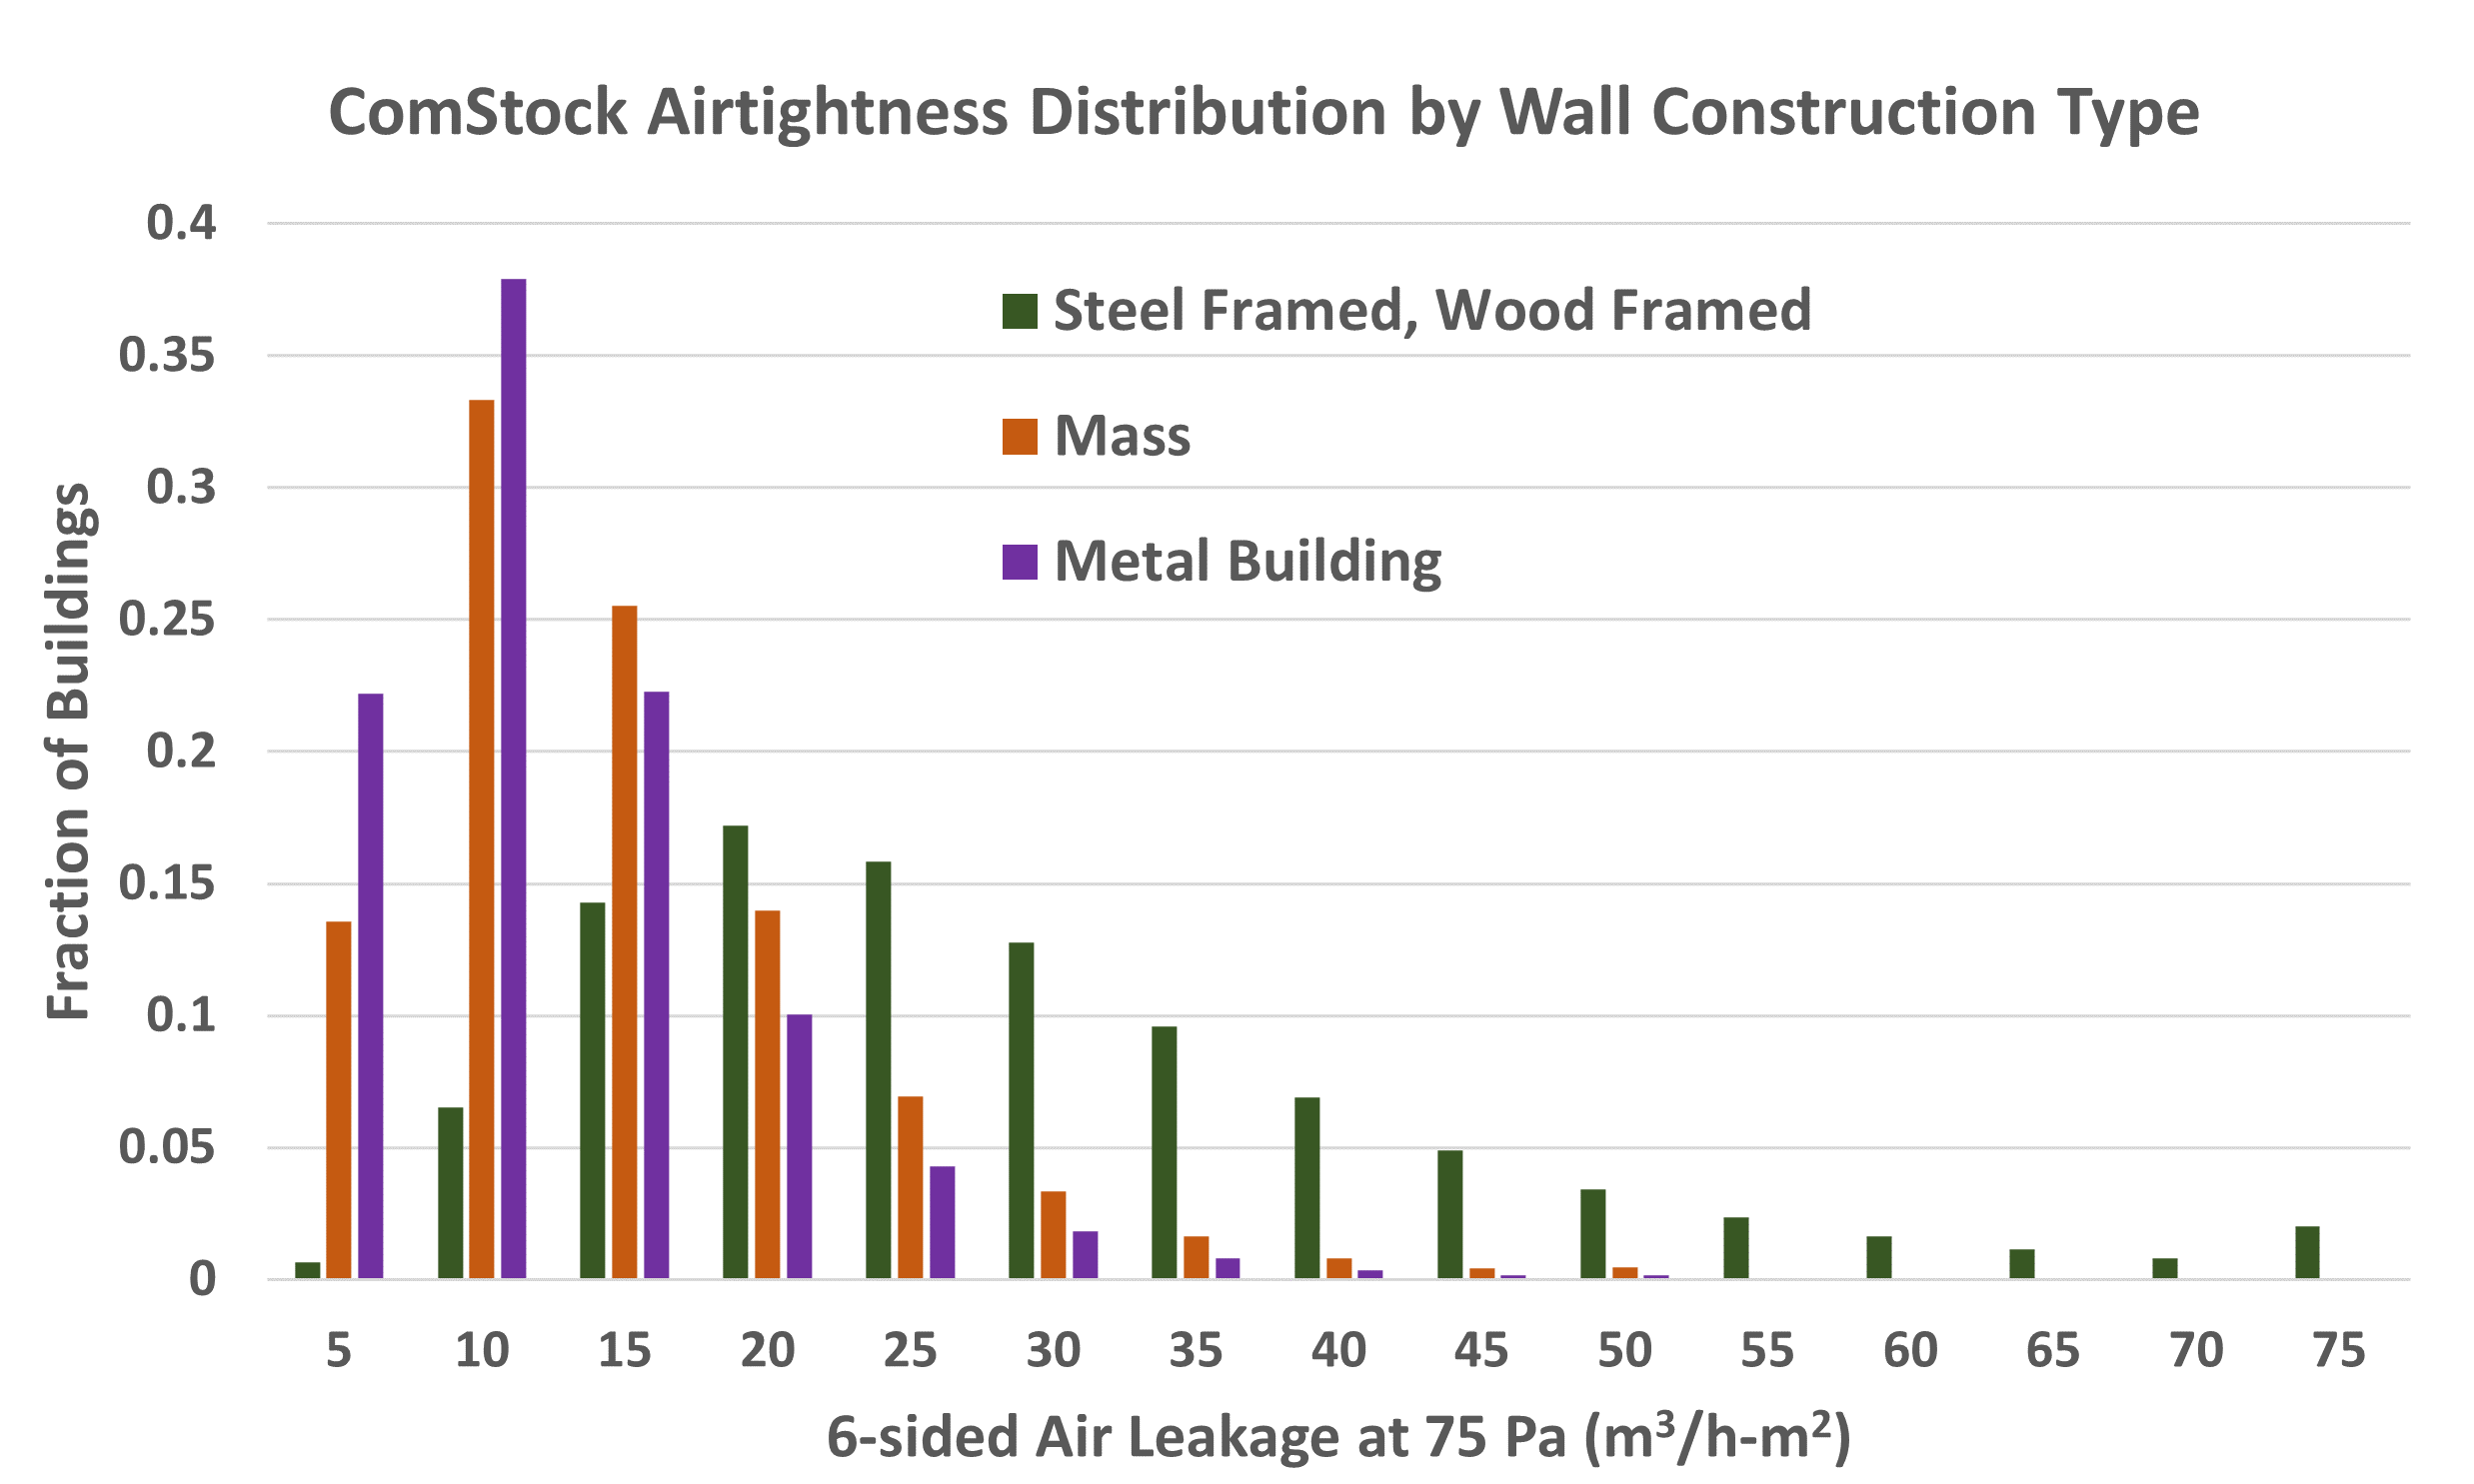
\includegraphics[width=0.9\textwidth]{figures/airtightness_by_wall_construction_type.png}
    \caption[Airtightness by Wall Construction Type]{6-sided airtightness distributions by wall construction type. Distributions are lognormal, with means matched to means by wall construction type in \citep{nist_infiltration_data}.}
    \label{fig:airtightness_by_wall_construction_type}
\end{figure}

\subsubsection{Infiltration Coefficients}
NIST derived coefficients by building CONTAM models of all of the DOE prototype buildings, as explained in \citep{nist_infiltration_correlations}. The coefficients assume a 4 Pa design pressure. The coefficients include A, B, and D terms, with C being 0. Coefficients are by building type, with separate coefficients for whether the HVAC system is on or off. The NIST report includes separate coefficients for buildings with air barriers, but ComStock does not assume buildings have air barriers.

NIST did not model all DOE prototype buildings, and does not include HVAC system off coefficients for some buildings if the prototype was modeled as always on. ComStock building types not available in the NIST data use coefficients for either the Office or Retail building types. If off coefficients are not available, the building uses the on coefficients instead.
\subsubsection{Natural Ventilation}

Natural ventilation is not modeled in ComStock because it is not common in the building stock.
